\setchapterpreamble[u]{\margintoc}
\chapter{Magnetic Field}

In this chapter we will cover what happens to the hydrogen atom when we include a magnetic field, we will start introducing what are the effects on a charge particle with a magnetic field.

\section{Introduction}

The magnetic field, $\vec{B}$, acts on a particle by the Lorentz Force:

\begin{equation}
  F = q \vec{v} \times \vec{B}
\end{equation}

Let's solve the problem for a particle with charge $e$, mass $m$, and velocity $\vec{v}$, in a constant magnetic field $\vec{B}$. We are going to set the z direction to be the direction of the magnetic field.

\begin{equation}
  \begin{array}{c}
    m \frac{d\vec{v}}{dt} = e \vec{v} \times \vec{B}
    \\

    \\
    \frac{d\vec{v}}{dt} = \frac{e B}{m} (-v_x \hat{y} + v_y \hat{x})
    \\

    \\
    \frac{dv_x}{dt} = \frac{eB}{m} v_y
    \\

    \\
    \frac{dv_y}{dt} = - \frac{eB}{m} v_x
    \\

    \\
    \frac{dv_z}{dt} = 0
    \\

    \\
    \vec{v} = v_0 \left[\sin(\omega t)\hat{x}+\cos(\omega t)\hat{y}\right]
    \\

    \\
    \vec{r} = \frac{v_0}{\omega}\left[-\cos(\omega t)\hat{x} + sin(\omega t) \hat{y}\right]
  \end{array}
\end{equation}

This represents a circular motion. The angular momentum of this motion is going to be:

\begin{equation}
  \begin{array}{c}
    \vec{L} = m \vec{r} \times \vec{v}
    \\

    \\
    \vec{L} = m \frac{v_0^2}{\omega} \hat{z}
    \\

    \\
    \vec{L} = \frac{mv_0^2}{eB/m} \hat{z} = \frac{m^2v_0^2}{eB} \hat{z}
  \end{array}
\end{equation}

The kinetic energy due to this magnetic field:

\begin{equation}
\frac{1}{2}mv_0^2 = \frac{1}{2} \frac{e}{m} \vec{L} \cdot \vec{B}
\end{equation}

The total energy is:

\begin{equation}
  \begin{array}{c}
    E = \frac{p^2}{2m} + V(r) + \frac{1}{2} \frac{e}{m} \vec{L} \cdot \vec{B}
    \\

    \\
    E = \frac{p^2}{2m} +V(r) + \mu \vec{L} \cdot \vec{B}
  \end{array}
\end{equation}

\section{Wave Equation}

The wave equation with this new term looks like:

\begin{equation}
  i\hbar\frac{\partial}{\partial t}\psi = \left[\frac{-\hbar^2}{2m}\left(\frac{\partial^2}{\partial x^2}+\frac{\partial^2}{\partial y^2}+\frac{\partial^2}{\partial z^2}\right)+V(r)+\mu \vec{L}\cdot\vec{B}\right]\psi
\end{equation}

If we called H to the first two terms, wecan still say that:

\begin{equation}
  \begin{array}{c}
    \left[H,L^2\right] = 0
    \\

    \\
    \left[H,L_z\right] = 0
    \\

    \\
    \left[L^2,L_z\right] = 0
  \end{array}
\end{equation}

We have that psi is a function over all space, so we can called it $\psi(r,\theta,\phi)$ with indices n,j,m.

\begin{equation}
  \begin{array}{c}
    L_z \psi_{n,j,m}(r,\theta,\phi) = \hbar m \psi_{n,j,m}(r,\theta,\phi)
    \\

    \\
    L^2 \psi_{n,j,m}(r,\theta,\phi) = \hbar^2 j(j+1) \psi_{n,j,m}(r,\theta,\phi)
    \\

    \\
    H \psi_{n,j,m}(r,\theta,\phi) = \left(-\frac{1}{2}\left(\frac{Ze^2}{4\pi\epsilon_0}\right)^2\frac{m}{\hbar^2 n^2}\right)\psi_{n,j,m}(r,\theta,\phi) = E_{n,j,m} \psi_{n,j,m}(r,\theta,\phi)
  \end{array}
\end{equation}

Our solution is an eigenfunction of H,L and $L^2$ simultaneously so we will say:

\begin{equation}
  \psi_{n,j,m}(r,\theta,\phi) \equiv \ket{n,j,m}
\end{equation}

Where:

\begin{equation}
  \braket{n_1,j_1,m_1}{n_2,j_2,m_2} = \delta_{n_1,n_2}\delta_{j_1,j_2}\delta_{m_1,m_2}
\end{equation}

If we continue with the assumption that B is in the z direction:

\begin{equation}
  \vec{L}\cdot\vec{B} = L_z B
\end{equation}

We define a new operator:

\begin{equation}
  H_B = H + \frac{eB}{2m} L_z
\end{equation}

If we applied this operator over the eigenfunction, we will get:

\begin{equation}
  \begin{array}{c}
    H_B \ket{n,j,m} = H\ket{n,j,m} + \frac{eB}{2m} L_z \ket{n,j,m}
    \\

    \\
    H_B \ket{n,j,m} = E_n \ket{n,j,m} + \frac{eB}{2m} \hbar m \ket{n,j,m}
    \\

    \\
    H_B \ket{n,j,m} = \left(E_n + \frac{eB}{2m} \hbar m\right) \ket{n,j,m}
  \end{array}
\end{equation}

This eigenvectors are just our solution for the hydrogen atom without a field shifted by a shift that depends on m.

\begin{figure}[H]
  \centering
  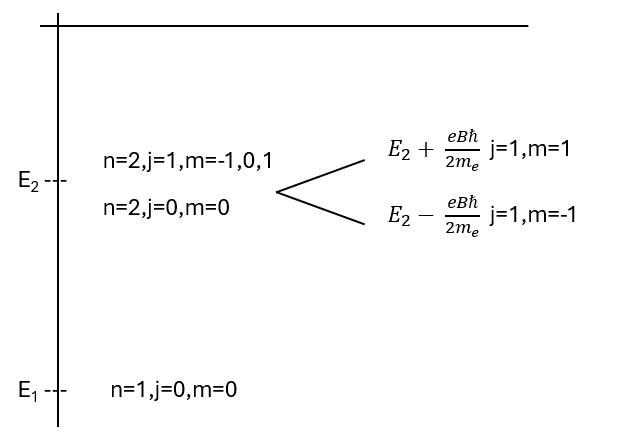
\includegraphics{images10/energy.PNG}
  \caption{Energy levels of the hydrogen atom with a magnetic field.}
\end{figure}
